\documentclass[twoside]{book}

% Packages required by doxygen
\usepackage{calc}
\usepackage{doxygen}
\usepackage{graphicx}
\usepackage[utf8]{inputenc}
\usepackage{makeidx}
\usepackage{multicol}
\usepackage{multirow}
\usepackage{textcomp}
\usepackage[table]{xcolor}

% Font selection
\usepackage[T1]{fontenc}
\usepackage{mathptmx}
\usepackage[scaled=.90]{helvet}
\usepackage{courier}
\usepackage{amssymb}
\usepackage{sectsty}
\renewcommand{\familydefault}{\sfdefault}
\allsectionsfont{%
  \fontseries{bc}\selectfont%
  \color{darkgray}%
}
\renewcommand{\DoxyLabelFont}{%
  \fontseries{bc}\selectfont%
  \color{darkgray}%
}

% Page & text layout
\usepackage{geometry}
\geometry{%
  a4paper,%
  top=2.5cm,%
  bottom=2.5cm,%
  left=2.5cm,%
  right=2.5cm%
}
\tolerance=750
\hfuzz=15pt
\hbadness=750
\setlength{\emergencystretch}{15pt}
\setlength{\parindent}{0cm}
\setlength{\parskip}{0.2cm}
\makeatletter
\renewcommand{\paragraph}{%
  \@startsection{paragraph}{4}{0ex}{-1.0ex}{1.0ex}{%
    \normalfont\normalsize\bfseries\SS@parafont%
  }%
}
\renewcommand{\subparagraph}{%
  \@startsection{subparagraph}{5}{0ex}{-1.0ex}{1.0ex}{%
    \normalfont\normalsize\bfseries\SS@subparafont%
  }%
}
\makeatother

% Headers & footers
\usepackage{fancyhdr}
\pagestyle{fancyplain}
\fancyhead[LE]{\fancyplain{}{\bfseries\thepage}}
\fancyhead[CE]{\fancyplain{}{}}
\fancyhead[RE]{\fancyplain{}{\bfseries\leftmark}}
\fancyhead[LO]{\fancyplain{}{\bfseries\rightmark}}
\fancyhead[CO]{\fancyplain{}{}}
\fancyhead[RO]{\fancyplain{}{\bfseries\thepage}}
\fancyfoot[LE]{\fancyplain{}{}}
\fancyfoot[CE]{\fancyplain{}{}}
\fancyfoot[RE]{\fancyplain{}{\bfseries\scriptsize Generated on Sun Jan 4 2015 15\-:10\-:07 for Jnthn-\/\-Lib by Doxygen }}
\fancyfoot[LO]{\fancyplain{}{\bfseries\scriptsize Generated on Sun Jan 4 2015 15\-:10\-:07 for Jnthn-\/\-Lib by Doxygen }}
\fancyfoot[CO]{\fancyplain{}{}}
\fancyfoot[RO]{\fancyplain{}{}}
\renewcommand{\footrulewidth}{0.4pt}
\renewcommand{\chaptermark}[1]{%
  \markboth{#1}{}%
}
\renewcommand{\sectionmark}[1]{%
  \markright{\thesection\ #1}%
}

% Indices & bibliography
\usepackage{natbib}
\usepackage[titles]{tocloft}
\setcounter{tocdepth}{3}
\setcounter{secnumdepth}{5}
\makeindex

% Hyperlinks (required, but should be loaded last)
\usepackage{ifpdf}
\ifpdf
  \usepackage[pdftex,pagebackref=true]{hyperref}
\else
  \usepackage[ps2pdf,pagebackref=true]{hyperref}
\fi
\hypersetup{%
  colorlinks=true,%
  linkcolor=blue,%
  citecolor=blue,%
  unicode%
}

% Custom commands
\newcommand{\clearemptydoublepage}{%
  \newpage{\pagestyle{empty}\cleardoublepage}%
}


%===== C O N T E N T S =====

\begin{document}

% Titlepage & ToC
\hypersetup{pageanchor=false}
\pagenumbering{roman}
\begin{titlepage}
\vspace*{7cm}
\begin{center}%
{\Large Jnthn-\/\-Lib }\\
\vspace*{1cm}
{\large Generated by Doxygen 1.8.6}\\
\vspace*{0.5cm}
{\small Sun Jan 4 2015 15:10:07}\\
\end{center}
\end{titlepage}
\clearemptydoublepage
\tableofcontents
\clearemptydoublepage
\pagenumbering{arabic}
\hypersetup{pageanchor=true}

%--- Begin generated contents ---
\chapter{Namespace Index}
\section{Namespace List}
Here is a list of all namespaces with brief descriptions\-:\begin{DoxyCompactList}
\item\contentsline{section}{\hyperlink{namespacejnthn}{jnthn} }{\pageref{namespacejnthn}}{}
\item\contentsline{section}{\hyperlink{namespacejnthn_1_1math}{jnthn\-::math} }{\pageref{namespacejnthn_1_1math}}{}
\item\contentsline{section}{\hyperlink{namespacejnthn_1_1stream}{jnthn\-::stream} }{\pageref{namespacejnthn_1_1stream}}{}
\end{DoxyCompactList}

\chapter{Hierarchical Index}
\section{Class Hierarchy}
This inheritance list is sorted roughly, but not completely, alphabetically\-:\begin{DoxyCompactList}
\item \contentsline{section}{jnthn\-:\-:stream\-:\-:Promise$<$ num $>$}{\pageref{classjnthn_1_1stream_1_1Promise}}{}
\begin{DoxyCompactList}
\item \contentsline{section}{jnthn\-:\-:stream\-:\-:Fil\-Promise$<$ num $>$}{\pageref{classjnthn_1_1stream_1_1FilPromise}}{}
\item \contentsline{section}{jnthn\-:\-:stream\-:\-:Num\-Promise$<$ num $>$}{\pageref{classjnthn_1_1stream_1_1NumPromise}}{}
\begin{DoxyCompactList}
\item \contentsline{section}{jnthn\-:\-:stream\-:\-:Fun\-Promise$<$ num $>$}{\pageref{classjnthn_1_1stream_1_1FunPromise}}{}
\end{DoxyCompactList}
\end{DoxyCompactList}
\item \contentsline{section}{jnthn\-:\-:stream\-:\-:Stream$<$ num $>$}{\pageref{classjnthn_1_1stream_1_1Stream}}{}
\item \contentsline{section}{jnthn\-:\-:math\-:\-:Vector}{\pageref{classjnthn_1_1math_1_1Vector}}{}
\end{DoxyCompactList}

\chapter{Class Index}
\section{Class List}
Here are the classes, structs, unions and interfaces with brief descriptions\-:\begin{DoxyCompactList}
\item\contentsline{section}{\hyperlink{classjnthn_1_1stream_1_1FilPromise}{jnthn\-::stream\-::\-Fil\-Promise$<$ num $>$} }{\pageref{classjnthn_1_1stream_1_1FilPromise}}{}
\item\contentsline{section}{\hyperlink{classjnthn_1_1stream_1_1FunPromise}{jnthn\-::stream\-::\-Fun\-Promise$<$ num $>$} }{\pageref{classjnthn_1_1stream_1_1FunPromise}}{}
\item\contentsline{section}{\hyperlink{classjnthn_1_1stream_1_1NumPromise}{jnthn\-::stream\-::\-Num\-Promise$<$ num $>$} }{\pageref{classjnthn_1_1stream_1_1NumPromise}}{}
\item\contentsline{section}{\hyperlink{classjnthn_1_1stream_1_1Promise}{jnthn\-::stream\-::\-Promise$<$ num $>$} }{\pageref{classjnthn_1_1stream_1_1Promise}}{}
\item\contentsline{section}{\hyperlink{classjnthn_1_1stream_1_1Stream}{jnthn\-::stream\-::\-Stream$<$ num $>$} }{\pageref{classjnthn_1_1stream_1_1Stream}}{}
\item\contentsline{section}{\hyperlink{classjnthn_1_1math_1_1Vector}{jnthn\-::math\-::\-Vector} }{\pageref{classjnthn_1_1math_1_1Vector}}{}
\end{DoxyCompactList}

\chapter{File Index}
\section{File List}
Here is a list of all files with brief descriptions\-:\begin{DoxyCompactList}
\item\contentsline{section}{include/\hyperlink{Stream_8h}{Stream.\-h} }{\pageref{Stream_8h}}{}
\item\contentsline{section}{src/\hyperlink{math_8h}{math.\-h} }{\pageref{math_8h}}{}
\item\contentsline{section}{src/\hyperlink{Stream_8cpp}{Stream.\-cpp} }{\pageref{Stream_8cpp}}{}
\item\contentsline{section}{src/\hyperlink{vector_8cpp}{vector.\-cpp} }{\pageref{vector_8cpp}}{}
\item\contentsline{section}{src/\hyperlink{vector_8h}{vector.\-h} }{\pageref{vector_8h}}{}
\end{DoxyCompactList}

\chapter{Namespace Documentation}
\hypertarget{namespacejnthn}{\section{jnthn Namespace Reference}
\label{namespacejnthn}\index{jnthn@{jnthn}}
}
\subsection*{Namespaces}
\begin{DoxyCompactItemize}
\item 
\hyperlink{namespacejnthn_1_1math}{math}
\item 
\hyperlink{namespacejnthn_1_1stream}{stream}
\end{DoxyCompactItemize}

\hypertarget{namespacejnthn_1_1math}{\section{jnthn\-:\-:math Namespace Reference}
\label{namespacejnthn_1_1math}\index{jnthn\-::math@{jnthn\-::math}}
}
\subsection*{Classes}
\begin{DoxyCompactItemize}
\item 
class \hyperlink{classjnthn_1_1math_1_1Vector}{Vector}
\end{DoxyCompactItemize}
\subsection*{Typedefs}
\begin{DoxyCompactItemize}
\item 
typedef int \hyperlink{namespacejnthn_1_1math_a5d3a263452a9caabf22cbb66cec013e9}{num}
\end{DoxyCompactItemize}


\subsection{Typedef Documentation}
\hypertarget{namespacejnthn_1_1math_a5d3a263452a9caabf22cbb66cec013e9}{\index{jnthn\-::math@{jnthn\-::math}!num@{num}}
\index{num@{num}!jnthn::math@{jnthn\-::math}}
\subsubsection[{num}]{\setlength{\rightskip}{0pt plus 5cm}typedef int {\bf jnthn\-::math\-::num}}}\label{namespacejnthn_1_1math_a5d3a263452a9caabf22cbb66cec013e9}

\hypertarget{namespacejnthn_1_1stream}{\section{jnthn\-:\-:stream Namespace Reference}
\label{namespacejnthn_1_1stream}\index{jnthn\-::stream@{jnthn\-::stream}}
}
\subsection*{Classes}
\begin{DoxyCompactItemize}
\item 
class \hyperlink{classjnthn_1_1stream_1_1Stream}{Stream}
\item 
class \hyperlink{classjnthn_1_1stream_1_1Promise}{Promise}
\item 
class \hyperlink{classjnthn_1_1stream_1_1NumPromise}{Num\-Promise}
\item 
class \hyperlink{classjnthn_1_1stream_1_1FunPromise}{Fun\-Promise}
\item 
class \hyperlink{classjnthn_1_1stream_1_1FilPromise}{Fil\-Promise}
\end{DoxyCompactItemize}

\chapter{Class Documentation}
\hypertarget{classjnthn_1_1stream_1_1FilPromise}{\section{jnthn\-:\-:stream\-:\-:Fil\-Promise$<$ num $>$ Class Template Reference}
\label{classjnthn_1_1stream_1_1FilPromise}\index{jnthn\-::stream\-::\-Fil\-Promise$<$ num $>$@{jnthn\-::stream\-::\-Fil\-Promise$<$ num $>$}}
}


{\ttfamily \#include $<$Stream.\-h$>$}

Inheritance diagram for jnthn\-:\-:stream\-:\-:Fil\-Promise$<$ num $>$\-:\begin{figure}[H]
\begin{center}
\leavevmode
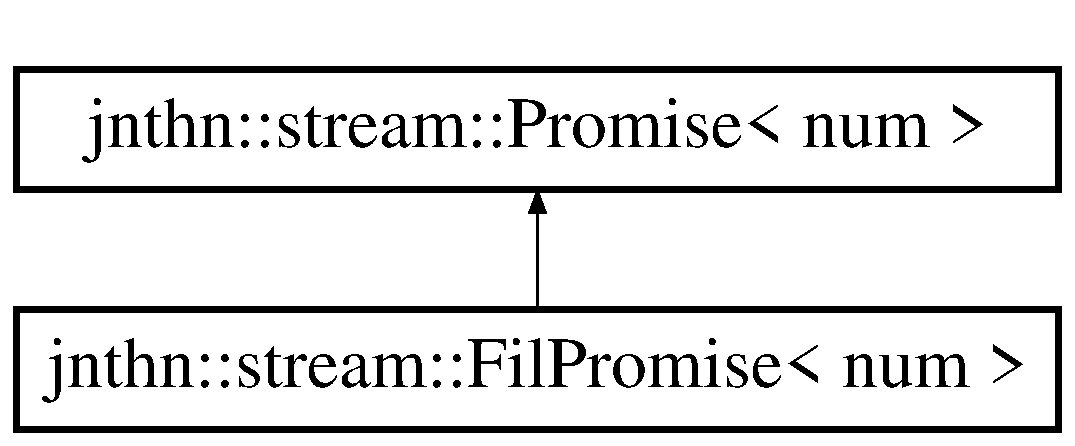
\includegraphics[height=2.000000cm]{classjnthn_1_1stream_1_1FilPromise}
\end{center}
\end{figure}
\subsection*{Public Types}
\begin{DoxyCompactItemize}
\item 
typedef bool($\ast$ \hyperlink{classjnthn_1_1stream_1_1FilPromise_a913328bcd089ed78816ed7b9a48f451c}{function} )(num value)
\end{DoxyCompactItemize}
\subsection*{Public Member Functions}
\begin{DoxyCompactItemize}
\item 
\hyperlink{classjnthn_1_1stream_1_1FilPromise_ab3e35d4eda1d20693de6705288b4d8a0}{Fil\-Promise} (\hyperlink{classjnthn_1_1stream_1_1Promise}{Promise}$<$ num $>$ $\ast$\hyperlink{classjnthn_1_1stream_1_1FilPromise_a96afb6c0553a74adf34c1fc2985e7c7e}{data}, \hyperlink{classjnthn_1_1stream_1_1FilPromise}{Fil\-Promise}$<$ num $>$\-::\hyperlink{classjnthn_1_1stream_1_1FilPromise_a913328bcd089ed78816ed7b9a48f451c}{function} \hyperlink{classjnthn_1_1stream_1_1FilPromise_abc2f868bf42fad27cda77e62d2b76cc7}{filter})
\item 
virtual num \hyperlink{classjnthn_1_1stream_1_1FilPromise_aa71b7543a7d2a080ba9e731f282d4c75}{get\-Data} ()
\item 
virtual \hyperlink{classjnthn_1_1stream_1_1Promise}{Promise}$<$ num $>$ $\ast$ \hyperlink{classjnthn_1_1stream_1_1FilPromise_a2cdd5bfff7be499272eedd5103890580}{get\-Next} ()
\end{DoxyCompactItemize}
\subsection*{Protected Attributes}
\begin{DoxyCompactItemize}
\item 
\hyperlink{classjnthn_1_1stream_1_1FilPromise_a913328bcd089ed78816ed7b9a48f451c}{function} \hyperlink{classjnthn_1_1stream_1_1FilPromise_abc2f868bf42fad27cda77e62d2b76cc7}{filter}
\item 
\hyperlink{classjnthn_1_1stream_1_1Promise}{Promise}$<$ num $>$ $\ast$ \hyperlink{classjnthn_1_1stream_1_1FilPromise_a96afb6c0553a74adf34c1fc2985e7c7e}{data}
\end{DoxyCompactItemize}


\subsection{Member Typedef Documentation}
\hypertarget{classjnthn_1_1stream_1_1FilPromise_a913328bcd089ed78816ed7b9a48f451c}{\index{jnthn\-::stream\-::\-Fil\-Promise@{jnthn\-::stream\-::\-Fil\-Promise}!function@{function}}
\index{function@{function}!jnthn::stream::FilPromise@{jnthn\-::stream\-::\-Fil\-Promise}}
\subsubsection[{function}]{\setlength{\rightskip}{0pt plus 5cm}template$<$typename num$>$ typedef bool($\ast$ {\bf jnthn\-::stream\-::\-Fil\-Promise}$<$ num $>$\-::function)(num value)}}\label{classjnthn_1_1stream_1_1FilPromise_a913328bcd089ed78816ed7b9a48f451c}


\subsection{Constructor \& Destructor Documentation}
\hypertarget{classjnthn_1_1stream_1_1FilPromise_ab3e35d4eda1d20693de6705288b4d8a0}{\index{jnthn\-::stream\-::\-Fil\-Promise@{jnthn\-::stream\-::\-Fil\-Promise}!Fil\-Promise@{Fil\-Promise}}
\index{Fil\-Promise@{Fil\-Promise}!jnthn::stream::FilPromise@{jnthn\-::stream\-::\-Fil\-Promise}}
\subsubsection[{Fil\-Promise}]{\setlength{\rightskip}{0pt plus 5cm}template$<$typename num $>$ Fil\-Promise\-::\-Fil\-Promise (
\begin{DoxyParamCaption}
\item[{{\bf Promise}$<$ num $>$ $\ast$}]{data, }
\item[{{\bf Fil\-Promise}$<$ num $>$\-::{\bf function}}]{filter}
\end{DoxyParamCaption}
)}}\label{classjnthn_1_1stream_1_1FilPromise_ab3e35d4eda1d20693de6705288b4d8a0}


\subsection{Member Function Documentation}
\hypertarget{classjnthn_1_1stream_1_1FilPromise_aa71b7543a7d2a080ba9e731f282d4c75}{\index{jnthn\-::stream\-::\-Fil\-Promise@{jnthn\-::stream\-::\-Fil\-Promise}!get\-Data@{get\-Data}}
\index{get\-Data@{get\-Data}!jnthn::stream::FilPromise@{jnthn\-::stream\-::\-Fil\-Promise}}
\subsubsection[{get\-Data}]{\setlength{\rightskip}{0pt plus 5cm}template$<$typename num $>$ num Fil\-Promise\-::get\-Data (
\begin{DoxyParamCaption}
{}
\end{DoxyParamCaption}
)\hspace{0.3cm}{\ttfamily [virtual]}}}\label{classjnthn_1_1stream_1_1FilPromise_aa71b7543a7d2a080ba9e731f282d4c75}


Implements \hyperlink{classjnthn_1_1stream_1_1Promise_af38928d3d23181ac68cc4a75c28ce253}{jnthn\-::stream\-::\-Promise$<$ num $>$}.

\hypertarget{classjnthn_1_1stream_1_1FilPromise_a2cdd5bfff7be499272eedd5103890580}{\index{jnthn\-::stream\-::\-Fil\-Promise@{jnthn\-::stream\-::\-Fil\-Promise}!get\-Next@{get\-Next}}
\index{get\-Next@{get\-Next}!jnthn::stream::FilPromise@{jnthn\-::stream\-::\-Fil\-Promise}}
\subsubsection[{get\-Next}]{\setlength{\rightskip}{0pt plus 5cm}template$<$typename num $>$ {\bf Promise}$<$ num $>$ $\ast$ Fil\-Promise\-::get\-Next (
\begin{DoxyParamCaption}
{}
\end{DoxyParamCaption}
)\hspace{0.3cm}{\ttfamily [virtual]}}}\label{classjnthn_1_1stream_1_1FilPromise_a2cdd5bfff7be499272eedd5103890580}


Implements \hyperlink{classjnthn_1_1stream_1_1Promise_a83cb9bc924207558629fc5a2908d5216}{jnthn\-::stream\-::\-Promise$<$ num $>$}.



\subsection{Member Data Documentation}
\hypertarget{classjnthn_1_1stream_1_1FilPromise_a96afb6c0553a74adf34c1fc2985e7c7e}{\index{jnthn\-::stream\-::\-Fil\-Promise@{jnthn\-::stream\-::\-Fil\-Promise}!data@{data}}
\index{data@{data}!jnthn::stream::FilPromise@{jnthn\-::stream\-::\-Fil\-Promise}}
\subsubsection[{data}]{\setlength{\rightskip}{0pt plus 5cm}template$<$typename num$>$ {\bf Promise}$<$num$>$$\ast$ {\bf jnthn\-::stream\-::\-Fil\-Promise}$<$ num $>$\-::data\hspace{0.3cm}{\ttfamily [protected]}}}\label{classjnthn_1_1stream_1_1FilPromise_a96afb6c0553a74adf34c1fc2985e7c7e}
\hypertarget{classjnthn_1_1stream_1_1FilPromise_abc2f868bf42fad27cda77e62d2b76cc7}{\index{jnthn\-::stream\-::\-Fil\-Promise@{jnthn\-::stream\-::\-Fil\-Promise}!filter@{filter}}
\index{filter@{filter}!jnthn::stream::FilPromise@{jnthn\-::stream\-::\-Fil\-Promise}}
\subsubsection[{filter}]{\setlength{\rightskip}{0pt plus 5cm}template$<$typename num$>$ {\bf function} {\bf jnthn\-::stream\-::\-Fil\-Promise}$<$ num $>$\-::filter\hspace{0.3cm}{\ttfamily [protected]}}}\label{classjnthn_1_1stream_1_1FilPromise_abc2f868bf42fad27cda77e62d2b76cc7}


The documentation for this class was generated from the following files\-:\begin{DoxyCompactItemize}
\item 
include/\hyperlink{Stream_8h}{Stream.\-h}\item 
src/\hyperlink{Stream_8cpp}{Stream.\-cpp}\end{DoxyCompactItemize}

\hypertarget{classjnthn_1_1stream_1_1FunPromise}{\section{jnthn\-:\-:stream\-:\-:Fun\-Promise$<$ num $>$ Class Template Reference}
\label{classjnthn_1_1stream_1_1FunPromise}\index{jnthn\-::stream\-::\-Fun\-Promise$<$ num $>$@{jnthn\-::stream\-::\-Fun\-Promise$<$ num $>$}}
}


{\ttfamily \#include $<$Stream.\-h$>$}

Inheritance diagram for jnthn\-:\-:stream\-:\-:Fun\-Promise$<$ num $>$\-:\begin{figure}[H]
\begin{center}
\leavevmode
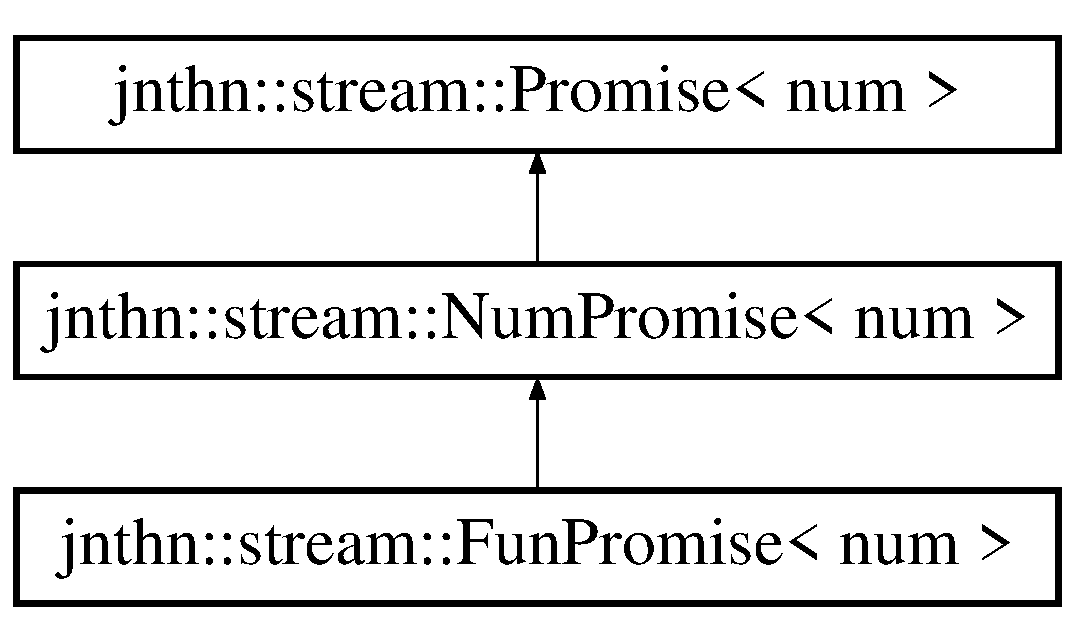
\includegraphics[height=3.000000cm]{classjnthn_1_1stream_1_1FunPromise}
\end{center}
\end{figure}
\subsection*{Public Types}
\begin{DoxyCompactItemize}
\item 
typedef num($\ast$ \hyperlink{classjnthn_1_1stream_1_1FunPromise_a23c79c18bfc402b4f2e6eb9de4bd3a37}{function} )(num \hyperlink{classjnthn_1_1stream_1_1NumPromise_a7d01e34ebf5e403ac4bf04139505d321}{domain})
\end{DoxyCompactItemize}
\subsection*{Public Member Functions}
\begin{DoxyCompactItemize}
\item 
\hyperlink{classjnthn_1_1stream_1_1FunPromise_af0355b7357b618a6d3cd219ef531f70d}{Fun\-Promise} (\hyperlink{classjnthn_1_1stream_1_1FunPromise_a23c79c18bfc402b4f2e6eb9de4bd3a37}{Fun\-Promise\-::function} \hyperlink{classjnthn_1_1stream_1_1NumPromise_a71f5507f8e605259eadb00417dbc2906}{fun}, num \hyperlink{classjnthn_1_1stream_1_1NumPromise_a7d01e34ebf5e403ac4bf04139505d321}{domain}, num \hyperlink{classjnthn_1_1stream_1_1FunPromise_a085f042b6a6290f177aaf73c2799b623}{delta}=1)
\item 
virtual num \hyperlink{classjnthn_1_1stream_1_1FunPromise_ab1dbc67a05202d73ac32524b92b0ef40}{get\-Data} ()
\item 
virtual \hyperlink{classjnthn_1_1stream_1_1Promise}{Promise}$<$ num $>$ $\ast$ \hyperlink{classjnthn_1_1stream_1_1FunPromise_a8c756f8b7dfc6304d82f1a514172d6fe}{get\-Next} ()
\end{DoxyCompactItemize}
\subsection*{Protected Attributes}
\begin{DoxyCompactItemize}
\item 
num \hyperlink{classjnthn_1_1stream_1_1FunPromise_a085f042b6a6290f177aaf73c2799b623}{delta}
\end{DoxyCompactItemize}


\subsection{Member Typedef Documentation}
\hypertarget{classjnthn_1_1stream_1_1FunPromise_a23c79c18bfc402b4f2e6eb9de4bd3a37}{\index{jnthn\-::stream\-::\-Fun\-Promise@{jnthn\-::stream\-::\-Fun\-Promise}!function@{function}}
\index{function@{function}!jnthn::stream::FunPromise@{jnthn\-::stream\-::\-Fun\-Promise}}
\subsubsection[{function}]{\setlength{\rightskip}{0pt plus 5cm}template$<$typename num $>$ typedef num($\ast$ {\bf jnthn\-::stream\-::\-Fun\-Promise}$<$ num $>$\-::function)(num {\bf domain})}}\label{classjnthn_1_1stream_1_1FunPromise_a23c79c18bfc402b4f2e6eb9de4bd3a37}


\subsection{Constructor \& Destructor Documentation}
\hypertarget{classjnthn_1_1stream_1_1FunPromise_af0355b7357b618a6d3cd219ef531f70d}{\index{jnthn\-::stream\-::\-Fun\-Promise@{jnthn\-::stream\-::\-Fun\-Promise}!Fun\-Promise@{Fun\-Promise}}
\index{Fun\-Promise@{Fun\-Promise}!jnthn::stream::FunPromise@{jnthn\-::stream\-::\-Fun\-Promise}}
\subsubsection[{Fun\-Promise}]{\setlength{\rightskip}{0pt plus 5cm}template$<$typename num $>$ Fun\-Promise\-::\-Fun\-Promise (
\begin{DoxyParamCaption}
\item[{{\bf Fun\-Promise}$<$ num $>$\-::{\bf function}}]{fun, }
\item[{num}]{domain, }
\item[{num}]{delta = {\ttfamily 1}}
\end{DoxyParamCaption}
)}}\label{classjnthn_1_1stream_1_1FunPromise_af0355b7357b618a6d3cd219ef531f70d}


\subsection{Member Function Documentation}
\hypertarget{classjnthn_1_1stream_1_1FunPromise_ab1dbc67a05202d73ac32524b92b0ef40}{\index{jnthn\-::stream\-::\-Fun\-Promise@{jnthn\-::stream\-::\-Fun\-Promise}!get\-Data@{get\-Data}}
\index{get\-Data@{get\-Data}!jnthn::stream::FunPromise@{jnthn\-::stream\-::\-Fun\-Promise}}
\subsubsection[{get\-Data}]{\setlength{\rightskip}{0pt plus 5cm}template$<$typename num $>$ num Fun\-Promise\-::get\-Data (
\begin{DoxyParamCaption}
{}
\end{DoxyParamCaption}
)\hspace{0.3cm}{\ttfamily [virtual]}}}\label{classjnthn_1_1stream_1_1FunPromise_ab1dbc67a05202d73ac32524b92b0ef40}


Implements \hyperlink{classjnthn_1_1stream_1_1NumPromise_a64b32eb3dd18b2b5eee79ef80a156a69}{jnthn\-::stream\-::\-Num\-Promise$<$ num $>$}.

\hypertarget{classjnthn_1_1stream_1_1FunPromise_a8c756f8b7dfc6304d82f1a514172d6fe}{\index{jnthn\-::stream\-::\-Fun\-Promise@{jnthn\-::stream\-::\-Fun\-Promise}!get\-Next@{get\-Next}}
\index{get\-Next@{get\-Next}!jnthn::stream::FunPromise@{jnthn\-::stream\-::\-Fun\-Promise}}
\subsubsection[{get\-Next}]{\setlength{\rightskip}{0pt plus 5cm}template$<$typename num $>$ {\bf Promise}$<$ num $>$ $\ast$ Fun\-Promise\-::get\-Next (
\begin{DoxyParamCaption}
{}
\end{DoxyParamCaption}
)\hspace{0.3cm}{\ttfamily [virtual]}}}\label{classjnthn_1_1stream_1_1FunPromise_a8c756f8b7dfc6304d82f1a514172d6fe}


Implements \hyperlink{classjnthn_1_1stream_1_1NumPromise_a3116d0c889cb2069c63d4e495de797e4}{jnthn\-::stream\-::\-Num\-Promise$<$ num $>$}.



\subsection{Member Data Documentation}
\hypertarget{classjnthn_1_1stream_1_1FunPromise_a085f042b6a6290f177aaf73c2799b623}{\index{jnthn\-::stream\-::\-Fun\-Promise@{jnthn\-::stream\-::\-Fun\-Promise}!delta@{delta}}
\index{delta@{delta}!jnthn::stream::FunPromise@{jnthn\-::stream\-::\-Fun\-Promise}}
\subsubsection[{delta}]{\setlength{\rightskip}{0pt plus 5cm}template$<$typename num $>$ num {\bf jnthn\-::stream\-::\-Fun\-Promise}$<$ num $>$\-::delta\hspace{0.3cm}{\ttfamily [protected]}}}\label{classjnthn_1_1stream_1_1FunPromise_a085f042b6a6290f177aaf73c2799b623}


The documentation for this class was generated from the following files\-:\begin{DoxyCompactItemize}
\item 
include/\hyperlink{Stream_8h}{Stream.\-h}\item 
src/\hyperlink{Stream_8cpp}{Stream.\-cpp}\end{DoxyCompactItemize}

\hypertarget{classjnthn_1_1stream_1_1NumPromise}{\section{jnthn\-:\-:stream\-:\-:Num\-Promise$<$ num $>$ Class Template Reference}
\label{classjnthn_1_1stream_1_1NumPromise}\index{jnthn\-::stream\-::\-Num\-Promise$<$ num $>$@{jnthn\-::stream\-::\-Num\-Promise$<$ num $>$}}
}


{\ttfamily \#include $<$Stream.\-h$>$}

Inheritance diagram for jnthn\-:\-:stream\-:\-:Num\-Promise$<$ num $>$\-:\begin{figure}[H]
\begin{center}
\leavevmode
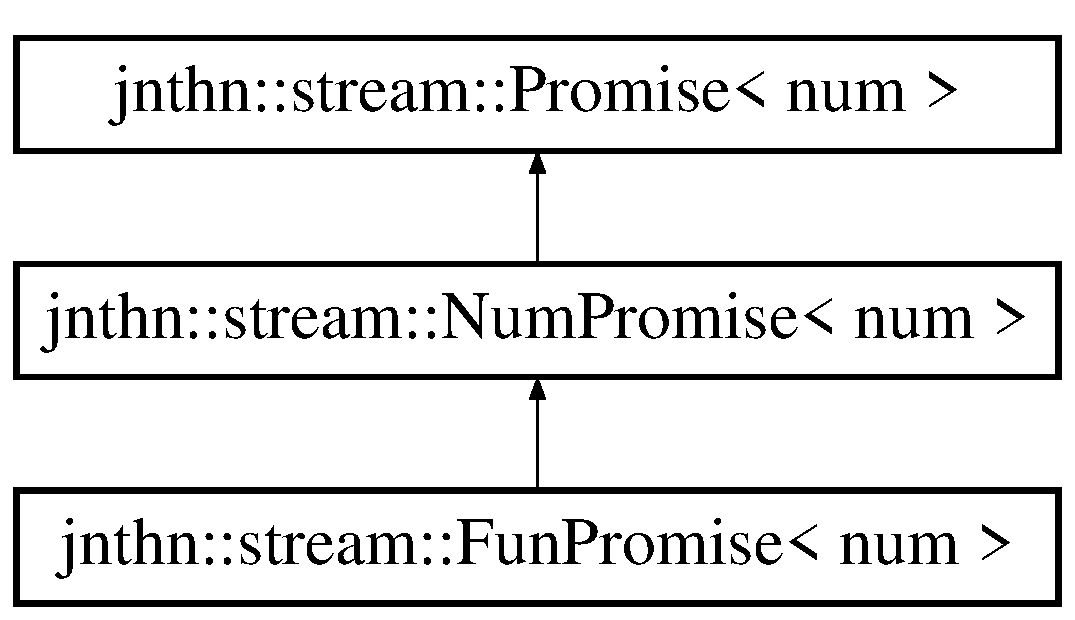
\includegraphics[height=3.000000cm]{classjnthn_1_1stream_1_1NumPromise}
\end{center}
\end{figure}
\subsection*{Public Types}
\begin{DoxyCompactItemize}
\item 
typedef num($\ast$ \hyperlink{classjnthn_1_1stream_1_1NumPromise_a362f41ffbe32df4763f4c35a56df295e}{function} )(num \hyperlink{classjnthn_1_1stream_1_1NumPromise_a7d01e34ebf5e403ac4bf04139505d321}{domain})
\end{DoxyCompactItemize}
\subsection*{Public Member Functions}
\begin{DoxyCompactItemize}
\item 
virtual num \hyperlink{classjnthn_1_1stream_1_1NumPromise_a64b32eb3dd18b2b5eee79ef80a156a69}{get\-Data} ()=0
\item 
virtual \hyperlink{classjnthn_1_1stream_1_1Promise}{Promise}$<$ num $>$ $\ast$ \hyperlink{classjnthn_1_1stream_1_1NumPromise_a3116d0c889cb2069c63d4e495de797e4}{get\-Next} ()=0
\end{DoxyCompactItemize}
\subsection*{Protected Attributes}
\begin{DoxyCompactItemize}
\item 
num \hyperlink{classjnthn_1_1stream_1_1NumPromise_a7d01e34ebf5e403ac4bf04139505d321}{domain}
\item 
\hyperlink{classjnthn_1_1stream_1_1NumPromise_a362f41ffbe32df4763f4c35a56df295e}{function} \hyperlink{classjnthn_1_1stream_1_1NumPromise_a71f5507f8e605259eadb00417dbc2906}{fun}
\end{DoxyCompactItemize}


\subsection{Member Typedef Documentation}
\hypertarget{classjnthn_1_1stream_1_1NumPromise_a362f41ffbe32df4763f4c35a56df295e}{\index{jnthn\-::stream\-::\-Num\-Promise@{jnthn\-::stream\-::\-Num\-Promise}!function@{function}}
\index{function@{function}!jnthn::stream::NumPromise@{jnthn\-::stream\-::\-Num\-Promise}}
\subsubsection[{function}]{\setlength{\rightskip}{0pt plus 5cm}template$<$typename num $>$ typedef num($\ast$ {\bf jnthn\-::stream\-::\-Num\-Promise}$<$ num $>$\-::function)(num {\bf domain})}}\label{classjnthn_1_1stream_1_1NumPromise_a362f41ffbe32df4763f4c35a56df295e}


\subsection{Member Function Documentation}
\hypertarget{classjnthn_1_1stream_1_1NumPromise_a64b32eb3dd18b2b5eee79ef80a156a69}{\index{jnthn\-::stream\-::\-Num\-Promise@{jnthn\-::stream\-::\-Num\-Promise}!get\-Data@{get\-Data}}
\index{get\-Data@{get\-Data}!jnthn::stream::NumPromise@{jnthn\-::stream\-::\-Num\-Promise}}
\subsubsection[{get\-Data}]{\setlength{\rightskip}{0pt plus 5cm}template$<$typename num $>$ virtual num {\bf jnthn\-::stream\-::\-Num\-Promise}$<$ num $>$\-::get\-Data (
\begin{DoxyParamCaption}
{}
\end{DoxyParamCaption}
)\hspace{0.3cm}{\ttfamily [pure virtual]}}}\label{classjnthn_1_1stream_1_1NumPromise_a64b32eb3dd18b2b5eee79ef80a156a69}


Implements \hyperlink{classjnthn_1_1stream_1_1Promise_af38928d3d23181ac68cc4a75c28ce253}{jnthn\-::stream\-::\-Promise$<$ num $>$}.



Implemented in \hyperlink{classjnthn_1_1stream_1_1FunPromise_ab1dbc67a05202d73ac32524b92b0ef40}{jnthn\-::stream\-::\-Fun\-Promise$<$ num $>$}.

\hypertarget{classjnthn_1_1stream_1_1NumPromise_a3116d0c889cb2069c63d4e495de797e4}{\index{jnthn\-::stream\-::\-Num\-Promise@{jnthn\-::stream\-::\-Num\-Promise}!get\-Next@{get\-Next}}
\index{get\-Next@{get\-Next}!jnthn::stream::NumPromise@{jnthn\-::stream\-::\-Num\-Promise}}
\subsubsection[{get\-Next}]{\setlength{\rightskip}{0pt plus 5cm}template$<$typename num $>$ virtual {\bf Promise}$<$num$>$$\ast$ {\bf jnthn\-::stream\-::\-Num\-Promise}$<$ num $>$\-::get\-Next (
\begin{DoxyParamCaption}
{}
\end{DoxyParamCaption}
)\hspace{0.3cm}{\ttfamily [pure virtual]}}}\label{classjnthn_1_1stream_1_1NumPromise_a3116d0c889cb2069c63d4e495de797e4}


Implements \hyperlink{classjnthn_1_1stream_1_1Promise_a83cb9bc924207558629fc5a2908d5216}{jnthn\-::stream\-::\-Promise$<$ num $>$}.



Implemented in \hyperlink{classjnthn_1_1stream_1_1FunPromise_a8c756f8b7dfc6304d82f1a514172d6fe}{jnthn\-::stream\-::\-Fun\-Promise$<$ num $>$}.



\subsection{Member Data Documentation}
\hypertarget{classjnthn_1_1stream_1_1NumPromise_a7d01e34ebf5e403ac4bf04139505d321}{\index{jnthn\-::stream\-::\-Num\-Promise@{jnthn\-::stream\-::\-Num\-Promise}!domain@{domain}}
\index{domain@{domain}!jnthn::stream::NumPromise@{jnthn\-::stream\-::\-Num\-Promise}}
\subsubsection[{domain}]{\setlength{\rightskip}{0pt plus 5cm}template$<$typename num $>$ num {\bf jnthn\-::stream\-::\-Num\-Promise}$<$ num $>$\-::domain\hspace{0.3cm}{\ttfamily [protected]}}}\label{classjnthn_1_1stream_1_1NumPromise_a7d01e34ebf5e403ac4bf04139505d321}
\hypertarget{classjnthn_1_1stream_1_1NumPromise_a71f5507f8e605259eadb00417dbc2906}{\index{jnthn\-::stream\-::\-Num\-Promise@{jnthn\-::stream\-::\-Num\-Promise}!fun@{fun}}
\index{fun@{fun}!jnthn::stream::NumPromise@{jnthn\-::stream\-::\-Num\-Promise}}
\subsubsection[{fun}]{\setlength{\rightskip}{0pt plus 5cm}template$<$typename num $>$ {\bf function} {\bf jnthn\-::stream\-::\-Num\-Promise}$<$ num $>$\-::fun\hspace{0.3cm}{\ttfamily [protected]}}}\label{classjnthn_1_1stream_1_1NumPromise_a71f5507f8e605259eadb00417dbc2906}


The documentation for this class was generated from the following file\-:\begin{DoxyCompactItemize}
\item 
include/\hyperlink{Stream_8h}{Stream.\-h}\end{DoxyCompactItemize}

\hypertarget{classjnthn_1_1stream_1_1Promise}{\section{jnthn\-:\-:stream\-:\-:Promise$<$ num $>$ Class Template Reference}
\label{classjnthn_1_1stream_1_1Promise}\index{jnthn\-::stream\-::\-Promise$<$ num $>$@{jnthn\-::stream\-::\-Promise$<$ num $>$}}
}


{\ttfamily \#include $<$Stream.\-h$>$}

Inheritance diagram for jnthn\-:\-:stream\-:\-:Promise$<$ num $>$\-:\begin{figure}[H]
\begin{center}
\leavevmode
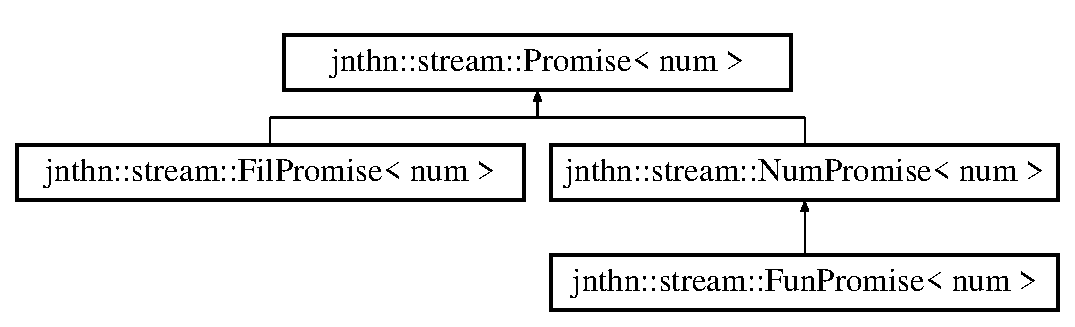
\includegraphics[height=3.000000cm]{classjnthn_1_1stream_1_1Promise}
\end{center}
\end{figure}
\subsection*{Public Member Functions}
\begin{DoxyCompactItemize}
\item 
virtual \hyperlink{classjnthn_1_1stream_1_1Promise}{Promise}$<$ num $>$ $\ast$ \hyperlink{classjnthn_1_1stream_1_1Promise_a83cb9bc924207558629fc5a2908d5216}{get\-Next} ()=0
\item 
virtual num \hyperlink{classjnthn_1_1stream_1_1Promise_af38928d3d23181ac68cc4a75c28ce253}{get\-Data} ()=0
\end{DoxyCompactItemize}
\subsection*{Protected Attributes}
\begin{DoxyCompactItemize}
\item 
bool \hyperlink{classjnthn_1_1stream_1_1Promise_ae1a23ef176aea5eac26c4d79a784b160}{collected}
\item 
bool \hyperlink{classjnthn_1_1stream_1_1Promise_a6b73728f5d4cbfe7ee23747fd5bcb98d}{generated}
\item 
num \hyperlink{classjnthn_1_1stream_1_1Promise_a189ef0405c6ddb48e4c204e242c2116b}{range}
\item 
\hyperlink{classjnthn_1_1stream_1_1Promise}{Promise}$<$ num $>$ $\ast$ \hyperlink{classjnthn_1_1stream_1_1Promise_a8c1da70608dd6397d0d0ad81c2db89e0}{nxt}
\end{DoxyCompactItemize}


\subsection{Member Function Documentation}
\hypertarget{classjnthn_1_1stream_1_1Promise_af38928d3d23181ac68cc4a75c28ce253}{\index{jnthn\-::stream\-::\-Promise@{jnthn\-::stream\-::\-Promise}!get\-Data@{get\-Data}}
\index{get\-Data@{get\-Data}!jnthn::stream::Promise@{jnthn\-::stream\-::\-Promise}}
\subsubsection[{get\-Data}]{\setlength{\rightskip}{0pt plus 5cm}template$<$typename num$>$ virtual num {\bf jnthn\-::stream\-::\-Promise}$<$ num $>$\-::get\-Data (
\begin{DoxyParamCaption}
{}
\end{DoxyParamCaption}
)\hspace{0.3cm}{\ttfamily [pure virtual]}}}\label{classjnthn_1_1stream_1_1Promise_af38928d3d23181ac68cc4a75c28ce253}


Implemented in \hyperlink{classjnthn_1_1stream_1_1FilPromise_aa71b7543a7d2a080ba9e731f282d4c75}{jnthn\-::stream\-::\-Fil\-Promise$<$ num $>$}, \hyperlink{classjnthn_1_1stream_1_1FunPromise_ab1dbc67a05202d73ac32524b92b0ef40}{jnthn\-::stream\-::\-Fun\-Promise$<$ num $>$}, and \hyperlink{classjnthn_1_1stream_1_1NumPromise_a64b32eb3dd18b2b5eee79ef80a156a69}{jnthn\-::stream\-::\-Num\-Promise$<$ num $>$}.

\hypertarget{classjnthn_1_1stream_1_1Promise_a83cb9bc924207558629fc5a2908d5216}{\index{jnthn\-::stream\-::\-Promise@{jnthn\-::stream\-::\-Promise}!get\-Next@{get\-Next}}
\index{get\-Next@{get\-Next}!jnthn::stream::Promise@{jnthn\-::stream\-::\-Promise}}
\subsubsection[{get\-Next}]{\setlength{\rightskip}{0pt plus 5cm}template$<$typename num$>$ virtual {\bf Promise}$<$num$>$$\ast$ {\bf jnthn\-::stream\-::\-Promise}$<$ num $>$\-::get\-Next (
\begin{DoxyParamCaption}
{}
\end{DoxyParamCaption}
)\hspace{0.3cm}{\ttfamily [pure virtual]}}}\label{classjnthn_1_1stream_1_1Promise_a83cb9bc924207558629fc5a2908d5216}


Implemented in \hyperlink{classjnthn_1_1stream_1_1FilPromise_a2cdd5bfff7be499272eedd5103890580}{jnthn\-::stream\-::\-Fil\-Promise$<$ num $>$}, \hyperlink{classjnthn_1_1stream_1_1FunPromise_a8c756f8b7dfc6304d82f1a514172d6fe}{jnthn\-::stream\-::\-Fun\-Promise$<$ num $>$}, and \hyperlink{classjnthn_1_1stream_1_1NumPromise_a3116d0c889cb2069c63d4e495de797e4}{jnthn\-::stream\-::\-Num\-Promise$<$ num $>$}.



\subsection{Member Data Documentation}
\hypertarget{classjnthn_1_1stream_1_1Promise_ae1a23ef176aea5eac26c4d79a784b160}{\index{jnthn\-::stream\-::\-Promise@{jnthn\-::stream\-::\-Promise}!collected@{collected}}
\index{collected@{collected}!jnthn::stream::Promise@{jnthn\-::stream\-::\-Promise}}
\subsubsection[{collected}]{\setlength{\rightskip}{0pt plus 5cm}template$<$typename num$>$ bool {\bf jnthn\-::stream\-::\-Promise}$<$ num $>$\-::collected\hspace{0.3cm}{\ttfamily [protected]}}}\label{classjnthn_1_1stream_1_1Promise_ae1a23ef176aea5eac26c4d79a784b160}
\hypertarget{classjnthn_1_1stream_1_1Promise_a6b73728f5d4cbfe7ee23747fd5bcb98d}{\index{jnthn\-::stream\-::\-Promise@{jnthn\-::stream\-::\-Promise}!generated@{generated}}
\index{generated@{generated}!jnthn::stream::Promise@{jnthn\-::stream\-::\-Promise}}
\subsubsection[{generated}]{\setlength{\rightskip}{0pt plus 5cm}template$<$typename num$>$ bool {\bf jnthn\-::stream\-::\-Promise}$<$ num $>$\-::generated\hspace{0.3cm}{\ttfamily [protected]}}}\label{classjnthn_1_1stream_1_1Promise_a6b73728f5d4cbfe7ee23747fd5bcb98d}
\hypertarget{classjnthn_1_1stream_1_1Promise_a8c1da70608dd6397d0d0ad81c2db89e0}{\index{jnthn\-::stream\-::\-Promise@{jnthn\-::stream\-::\-Promise}!nxt@{nxt}}
\index{nxt@{nxt}!jnthn::stream::Promise@{jnthn\-::stream\-::\-Promise}}
\subsubsection[{nxt}]{\setlength{\rightskip}{0pt plus 5cm}template$<$typename num$>$ {\bf Promise}$<$num$>$$\ast$ {\bf jnthn\-::stream\-::\-Promise}$<$ num $>$\-::nxt\hspace{0.3cm}{\ttfamily [protected]}}}\label{classjnthn_1_1stream_1_1Promise_a8c1da70608dd6397d0d0ad81c2db89e0}
\hypertarget{classjnthn_1_1stream_1_1Promise_a189ef0405c6ddb48e4c204e242c2116b}{\index{jnthn\-::stream\-::\-Promise@{jnthn\-::stream\-::\-Promise}!range@{range}}
\index{range@{range}!jnthn::stream::Promise@{jnthn\-::stream\-::\-Promise}}
\subsubsection[{range}]{\setlength{\rightskip}{0pt plus 5cm}template$<$typename num$>$ num {\bf jnthn\-::stream\-::\-Promise}$<$ num $>$\-::range\hspace{0.3cm}{\ttfamily [protected]}}}\label{classjnthn_1_1stream_1_1Promise_a189ef0405c6ddb48e4c204e242c2116b}


The documentation for this class was generated from the following file\-:\begin{DoxyCompactItemize}
\item 
include/\hyperlink{Stream_8h}{Stream.\-h}\end{DoxyCompactItemize}

\hypertarget{classjnthn_1_1stream_1_1Stream}{\section{jnthn\-:\-:stream\-:\-:Stream$<$ num $>$ Class Template Reference}
\label{classjnthn_1_1stream_1_1Stream}\index{jnthn\-::stream\-::\-Stream$<$ num $>$@{jnthn\-::stream\-::\-Stream$<$ num $>$}}
}


{\ttfamily \#include $<$Stream.\-h$>$}

\subsection*{Public Member Functions}
\begin{DoxyCompactItemize}
\item 
\hyperlink{classjnthn_1_1stream_1_1Stream_a37b7ae76fc92fec60d0af1c3ffc048ba}{Stream} (\hyperlink{classjnthn_1_1stream_1_1Promise}{Promise}$<$ num $>$ $\ast$p)
\item 
num \hyperlink{classjnthn_1_1stream_1_1Stream_a85a03b3a8508b49deda54e878fd421fd}{operator\mbox{[}$\,$\mbox{]}} (const int index)
\item 
\hyperlink{classjnthn_1_1stream_1_1Stream}{Stream} \& \hyperlink{classjnthn_1_1stream_1_1Stream_aa10977ba02642520a92a1bdfa633ef0f}{operator++} ()
\end{DoxyCompactItemize}


\subsection{Constructor \& Destructor Documentation}
\hypertarget{classjnthn_1_1stream_1_1Stream_a37b7ae76fc92fec60d0af1c3ffc048ba}{\index{jnthn\-::stream\-::\-Stream@{jnthn\-::stream\-::\-Stream}!Stream@{Stream}}
\index{Stream@{Stream}!jnthn::stream::Stream@{jnthn\-::stream\-::\-Stream}}
\subsubsection[{Stream}]{\setlength{\rightskip}{0pt plus 5cm}template$<$typename num $>$ Stream\-::\-Stream (
\begin{DoxyParamCaption}
\item[{{\bf Promise}$<$ num $>$ $\ast$}]{p}
\end{DoxyParamCaption}
)}}\label{classjnthn_1_1stream_1_1Stream_a37b7ae76fc92fec60d0af1c3ffc048ba}


\subsection{Member Function Documentation}
\hypertarget{classjnthn_1_1stream_1_1Stream_aa10977ba02642520a92a1bdfa633ef0f}{\index{jnthn\-::stream\-::\-Stream@{jnthn\-::stream\-::\-Stream}!operator++@{operator++}}
\index{operator++@{operator++}!jnthn::stream::Stream@{jnthn\-::stream\-::\-Stream}}
\subsubsection[{operator++}]{\setlength{\rightskip}{0pt plus 5cm}template$<$typename num $>$ {\bf Stream}\& {\bf jnthn\-::stream\-::\-Stream}$<$ num $>$\-::operator++ (
\begin{DoxyParamCaption}
{}
\end{DoxyParamCaption}
)\hspace{0.3cm}{\ttfamily [inline]}}}\label{classjnthn_1_1stream_1_1Stream_aa10977ba02642520a92a1bdfa633ef0f}
\hypertarget{classjnthn_1_1stream_1_1Stream_a85a03b3a8508b49deda54e878fd421fd}{\index{jnthn\-::stream\-::\-Stream@{jnthn\-::stream\-::\-Stream}!operator\mbox{[}$\,$\mbox{]}@{operator[]}}
\index{operator\mbox{[}$\,$\mbox{]}@{operator[]}!jnthn::stream::Stream@{jnthn\-::stream\-::\-Stream}}
\subsubsection[{operator[]}]{\setlength{\rightskip}{0pt plus 5cm}template$<$typename num $>$ num Stream\-::operator\mbox{[}$\,$\mbox{]} (
\begin{DoxyParamCaption}
\item[{const int}]{index}
\end{DoxyParamCaption}
)}}\label{classjnthn_1_1stream_1_1Stream_a85a03b3a8508b49deda54e878fd421fd}


The documentation for this class was generated from the following files\-:\begin{DoxyCompactItemize}
\item 
include/\hyperlink{Stream_8h}{Stream.\-h}\item 
src/\hyperlink{Stream_8cpp}{Stream.\-cpp}\end{DoxyCompactItemize}

\hypertarget{classjnthn_1_1math_1_1Vector}{\section{jnthn\-:\-:math\-:\-:Vector Class Reference}
\label{classjnthn_1_1math_1_1Vector}\index{jnthn\-::math\-::\-Vector@{jnthn\-::math\-::\-Vector}}
}


{\ttfamily \#include $<$vector.\-h$>$}

\subsection*{Public Member Functions}
\begin{DoxyCompactItemize}
\item 
\hyperlink{classjnthn_1_1math_1_1Vector_af2d199ef0c0d93168399cee3afb6dbfe}{Vector} (int size, \hyperlink{vector_8cpp_a65603216afa9e90437684d0557b6ecb3}{v\-Type} type=\hyperlink{vector_8cpp_a65603216afa9e90437684d0557b6ecb3ac5a3a4f3774bc6aff01acdbd9862a1a9}{C\-O\-L\-U\-M\-N})
\item 
\hyperlink{classjnthn_1_1math_1_1Vector_aff6df5703baab149feb10e6194e4ae62}{Vector} (\hyperlink{namespacejnthn_1_1math_a5d3a263452a9caabf22cbb66cec013e9}{num} $\ast$data, \hyperlink{vector_8cpp_a65603216afa9e90437684d0557b6ecb3}{v\-Type} type=\hyperlink{vector_8cpp_a65603216afa9e90437684d0557b6ecb3ac5a3a4f3774bc6aff01acdbd9862a1a9}{C\-O\-L\-U\-M\-N})
\item 
\hyperlink{classjnthn_1_1math_1_1Vector_a5a10aeadba061bca5d7adc45e1f0235d}{$\sim$\-Vector} ()
\item 
int \hyperlink{classjnthn_1_1math_1_1Vector_a29884418c42955e7f56561dae258727c}{get} (int index)
\item 
void \hyperlink{classjnthn_1_1math_1_1Vector_acd54269987bb1256ff3d65caba26b042}{set} (int index, \hyperlink{namespacejnthn_1_1math_a5d3a263452a9caabf22cbb66cec013e9}{num} value)
\item 
const \hyperlink{classjnthn_1_1math_1_1Vector}{Vector} \hyperlink{classjnthn_1_1math_1_1Vector_aedd5b6c15e1c323610c9843fa799d95f}{operator+} (const \hyperlink{classjnthn_1_1math_1_1Vector}{Vector} rvalue) const 
\item 
const \hyperlink{vector_8cpp_a65603216afa9e90437684d0557b6ecb3}{v\-Type} \hyperlink{classjnthn_1_1math_1_1Vector_aca060c98d44054aa10f5de8986a3a7ad}{get\-Type} ()
\item 
void \hyperlink{classjnthn_1_1math_1_1Vector_a4a11e9a32e7d48a5a0993456da0dce63}{set\-Type} (\hyperlink{vector_8cpp_a65603216afa9e90437684d0557b6ecb3}{v\-Type} type)
\item 
int \hyperlink{classjnthn_1_1math_1_1Vector_a1e58c0bbe1e20521275e4bacac1d4d6a}{get\-Length} ()
\end{DoxyCompactItemize}


\subsection{Constructor \& Destructor Documentation}
\hypertarget{classjnthn_1_1math_1_1Vector_af2d199ef0c0d93168399cee3afb6dbfe}{\index{jnthn\-::math\-::\-Vector@{jnthn\-::math\-::\-Vector}!Vector@{Vector}}
\index{Vector@{Vector}!jnthn::math::Vector@{jnthn\-::math\-::\-Vector}}
\subsubsection[{Vector}]{\setlength{\rightskip}{0pt plus 5cm}Vector\-::\-Vector (
\begin{DoxyParamCaption}
\item[{int}]{size, }
\item[{{\bf v\-Type}}]{type = {\ttfamily {\bf C\-O\-L\-U\-M\-N}}}
\end{DoxyParamCaption}
)}}\label{classjnthn_1_1math_1_1Vector_af2d199ef0c0d93168399cee3afb6dbfe}
\hypertarget{classjnthn_1_1math_1_1Vector_aff6df5703baab149feb10e6194e4ae62}{\index{jnthn\-::math\-::\-Vector@{jnthn\-::math\-::\-Vector}!Vector@{Vector}}
\index{Vector@{Vector}!jnthn::math::Vector@{jnthn\-::math\-::\-Vector}}
\subsubsection[{Vector}]{\setlength{\rightskip}{0pt plus 5cm}Vector\-::\-Vector (
\begin{DoxyParamCaption}
\item[{{\bf num} $\ast$}]{data, }
\item[{{\bf v\-Type}}]{type = {\ttfamily {\bf C\-O\-L\-U\-M\-N}}}
\end{DoxyParamCaption}
)}}\label{classjnthn_1_1math_1_1Vector_aff6df5703baab149feb10e6194e4ae62}
\hypertarget{classjnthn_1_1math_1_1Vector_a5a10aeadba061bca5d7adc45e1f0235d}{\index{jnthn\-::math\-::\-Vector@{jnthn\-::math\-::\-Vector}!$\sim$\-Vector@{$\sim$\-Vector}}
\index{$\sim$\-Vector@{$\sim$\-Vector}!jnthn::math::Vector@{jnthn\-::math\-::\-Vector}}
\subsubsection[{$\sim$\-Vector}]{\setlength{\rightskip}{0pt plus 5cm}jnthn\-::math\-::\-Vector\-::$\sim$\-Vector (
\begin{DoxyParamCaption}
{}
\end{DoxyParamCaption}
)}}\label{classjnthn_1_1math_1_1Vector_a5a10aeadba061bca5d7adc45e1f0235d}


\subsection{Member Function Documentation}
\hypertarget{classjnthn_1_1math_1_1Vector_a29884418c42955e7f56561dae258727c}{\index{jnthn\-::math\-::\-Vector@{jnthn\-::math\-::\-Vector}!get@{get}}
\index{get@{get}!jnthn::math::Vector@{jnthn\-::math\-::\-Vector}}
\subsubsection[{get}]{\setlength{\rightskip}{0pt plus 5cm}int Vector\-::get (
\begin{DoxyParamCaption}
\item[{int}]{index}
\end{DoxyParamCaption}
)}}\label{classjnthn_1_1math_1_1Vector_a29884418c42955e7f56561dae258727c}
\hypertarget{classjnthn_1_1math_1_1Vector_a1e58c0bbe1e20521275e4bacac1d4d6a}{\index{jnthn\-::math\-::\-Vector@{jnthn\-::math\-::\-Vector}!get\-Length@{get\-Length}}
\index{get\-Length@{get\-Length}!jnthn::math::Vector@{jnthn\-::math\-::\-Vector}}
\subsubsection[{get\-Length}]{\setlength{\rightskip}{0pt plus 5cm}int Vector\-::get\-Length (
\begin{DoxyParamCaption}
{}
\end{DoxyParamCaption}
)}}\label{classjnthn_1_1math_1_1Vector_a1e58c0bbe1e20521275e4bacac1d4d6a}
\hypertarget{classjnthn_1_1math_1_1Vector_aca060c98d44054aa10f5de8986a3a7ad}{\index{jnthn\-::math\-::\-Vector@{jnthn\-::math\-::\-Vector}!get\-Type@{get\-Type}}
\index{get\-Type@{get\-Type}!jnthn::math::Vector@{jnthn\-::math\-::\-Vector}}
\subsubsection[{get\-Type}]{\setlength{\rightskip}{0pt plus 5cm}const {\bf v\-Type} Vector\-::get\-Type (
\begin{DoxyParamCaption}
{}
\end{DoxyParamCaption}
)}}\label{classjnthn_1_1math_1_1Vector_aca060c98d44054aa10f5de8986a3a7ad}
\hypertarget{classjnthn_1_1math_1_1Vector_aedd5b6c15e1c323610c9843fa799d95f}{\index{jnthn\-::math\-::\-Vector@{jnthn\-::math\-::\-Vector}!operator+@{operator+}}
\index{operator+@{operator+}!jnthn::math::Vector@{jnthn\-::math\-::\-Vector}}
\subsubsection[{operator+}]{\setlength{\rightskip}{0pt plus 5cm}const {\bf Vector} Vector\-::operator+ (
\begin{DoxyParamCaption}
\item[{const {\bf Vector}}]{rvalue}
\end{DoxyParamCaption}
) const}}\label{classjnthn_1_1math_1_1Vector_aedd5b6c15e1c323610c9843fa799d95f}
\hypertarget{classjnthn_1_1math_1_1Vector_acd54269987bb1256ff3d65caba26b042}{\index{jnthn\-::math\-::\-Vector@{jnthn\-::math\-::\-Vector}!set@{set}}
\index{set@{set}!jnthn::math::Vector@{jnthn\-::math\-::\-Vector}}
\subsubsection[{set}]{\setlength{\rightskip}{0pt plus 5cm}void Vector\-::set (
\begin{DoxyParamCaption}
\item[{int}]{index, }
\item[{{\bf num}}]{value}
\end{DoxyParamCaption}
)}}\label{classjnthn_1_1math_1_1Vector_acd54269987bb1256ff3d65caba26b042}
\hypertarget{classjnthn_1_1math_1_1Vector_a4a11e9a32e7d48a5a0993456da0dce63}{\index{jnthn\-::math\-::\-Vector@{jnthn\-::math\-::\-Vector}!set\-Type@{set\-Type}}
\index{set\-Type@{set\-Type}!jnthn::math::Vector@{jnthn\-::math\-::\-Vector}}
\subsubsection[{set\-Type}]{\setlength{\rightskip}{0pt plus 5cm}void Vector\-::set\-Type (
\begin{DoxyParamCaption}
\item[{{\bf v\-Type}}]{type}
\end{DoxyParamCaption}
)}}\label{classjnthn_1_1math_1_1Vector_a4a11e9a32e7d48a5a0993456da0dce63}


The documentation for this class was generated from the following files\-:\begin{DoxyCompactItemize}
\item 
src/\hyperlink{vector_8h}{vector.\-h}\item 
src/\hyperlink{vector_8cpp}{vector.\-cpp}\end{DoxyCompactItemize}

\chapter{File Documentation}
\hypertarget{Stream_8h}{\section{include/\-Stream.h File Reference}
\label{Stream_8h}\index{include/\-Stream.\-h@{include/\-Stream.\-h}}
}
\subsection*{Classes}
\begin{DoxyCompactItemize}
\item 
class \hyperlink{classjnthn_1_1stream_1_1Stream}{jnthn\-::stream\-::\-Stream$<$ num $>$}
\item 
class \hyperlink{classjnthn_1_1stream_1_1Promise}{jnthn\-::stream\-::\-Promise$<$ num $>$}
\item 
class \hyperlink{classjnthn_1_1stream_1_1NumPromise}{jnthn\-::stream\-::\-Num\-Promise$<$ num $>$}
\item 
class \hyperlink{classjnthn_1_1stream_1_1FunPromise}{jnthn\-::stream\-::\-Fun\-Promise$<$ num $>$}
\item 
class \hyperlink{classjnthn_1_1stream_1_1FilPromise}{jnthn\-::stream\-::\-Fil\-Promise$<$ num $>$}
\item 
class \hyperlink{classjnthn_1_1stream_1_1Stream}{jnthn\-::stream\-::\-Stream$<$ num $>$}
\item 
class \hyperlink{classjnthn_1_1stream_1_1Promise}{jnthn\-::stream\-::\-Promise$<$ num $>$}
\item 
class \hyperlink{classjnthn_1_1stream_1_1NumPromise}{jnthn\-::stream\-::\-Num\-Promise$<$ num $>$}
\item 
class \hyperlink{classjnthn_1_1stream_1_1FunPromise}{jnthn\-::stream\-::\-Fun\-Promise$<$ num $>$}
\item 
class \hyperlink{classjnthn_1_1stream_1_1FilPromise}{jnthn\-::stream\-::\-Fil\-Promise$<$ num $>$}
\end{DoxyCompactItemize}
\subsection*{Namespaces}
\begin{DoxyCompactItemize}
\item 
\hyperlink{namespacejnthn}{jnthn}
\item 
\hyperlink{namespacejnthn_1_1stream}{jnthn\-::stream}
\end{DoxyCompactItemize}

\hypertarget{math_8h}{\section{src/math.h File Reference}
\label{math_8h}\index{src/math.\-h@{src/math.\-h}}
}
{\ttfamily \#include \char`\"{}vector.\-h\char`\"{}}\\*
\subsection*{Namespaces}
\begin{DoxyCompactItemize}
\item 
\hyperlink{namespacejnthn}{jnthn}
\item 
\hyperlink{namespacejnthn_1_1math}{jnthn\-::math}
\end{DoxyCompactItemize}
\subsection*{Typedefs}
\begin{DoxyCompactItemize}
\item 
typedef int \hyperlink{namespacejnthn_1_1math_a5d3a263452a9caabf22cbb66cec013e9}{jnthn\-::math\-::num}
\end{DoxyCompactItemize}

\hypertarget{Stream_8cpp}{\section{src/\-Stream.cpp File Reference}
\label{Stream_8cpp}\index{src/\-Stream.\-cpp@{src/\-Stream.\-cpp}}
}
{\ttfamily \#include \char`\"{}../include/\-Stream.\-h\char`\"{}}\\*

\hypertarget{vector_8cpp}{\section{src/vector.cpp File Reference}
\label{vector_8cpp}\index{src/vector.\-cpp@{src/vector.\-cpp}}
}
{\ttfamily \#include \char`\"{}vector.\-h\char`\"{}}\\*
\subsection*{Enumerations}
\begin{DoxyCompactItemize}
\item 
enum \hyperlink{vector_8cpp_a65603216afa9e90437684d0557b6ecb3}{v\-Type} \{ \hyperlink{vector_8cpp_a65603216afa9e90437684d0557b6ecb3abf470e461303b909bf0dc58084ebafa0}{R\-O\-W}, 
\hyperlink{vector_8cpp_a65603216afa9e90437684d0557b6ecb3ac5a3a4f3774bc6aff01acdbd9862a1a9}{C\-O\-L\-U\-M\-N}
 \}
\end{DoxyCompactItemize}


\subsection{Enumeration Type Documentation}
\hypertarget{vector_8cpp_a65603216afa9e90437684d0557b6ecb3}{\index{vector.\-cpp@{vector.\-cpp}!v\-Type@{v\-Type}}
\index{v\-Type@{v\-Type}!vector.cpp@{vector.\-cpp}}
\subsubsection[{v\-Type}]{\setlength{\rightskip}{0pt plus 5cm}enum {\bf v\-Type}}}\label{vector_8cpp_a65603216afa9e90437684d0557b6ecb3}
\begin{Desc}
\item[Enumerator]\par
\begin{description}
\index{R\-O\-W@{R\-O\-W}!vector.\-cpp@{vector.\-cpp}}\index{vector.\-cpp@{vector.\-cpp}!R\-O\-W@{R\-O\-W}}\item[{\em 
\hypertarget{vector_8cpp_a65603216afa9e90437684d0557b6ecb3abf470e461303b909bf0dc58084ebafa0}{R\-O\-W}\label{vector_8cpp_a65603216afa9e90437684d0557b6ecb3abf470e461303b909bf0dc58084ebafa0}
}]\index{C\-O\-L\-U\-M\-N@{C\-O\-L\-U\-M\-N}!vector.\-cpp@{vector.\-cpp}}\index{vector.\-cpp@{vector.\-cpp}!C\-O\-L\-U\-M\-N@{C\-O\-L\-U\-M\-N}}\item[{\em 
\hypertarget{vector_8cpp_a65603216afa9e90437684d0557b6ecb3ac5a3a4f3774bc6aff01acdbd9862a1a9}{C\-O\-L\-U\-M\-N}\label{vector_8cpp_a65603216afa9e90437684d0557b6ecb3ac5a3a4f3774bc6aff01acdbd9862a1a9}
}]\end{description}
\end{Desc}

\hypertarget{vector_8h}{\section{src/vector.h File Reference}
\label{vector_8h}\index{src/vector.\-h@{src/vector.\-h}}
}
\subsection*{Classes}
\begin{DoxyCompactItemize}
\item 
class \hyperlink{classjnthn_1_1math_1_1Vector}{jnthn\-::math\-::\-Vector}
\end{DoxyCompactItemize}
\subsection*{Namespaces}
\begin{DoxyCompactItemize}
\item 
\hyperlink{namespacejnthn}{jnthn}
\item 
\hyperlink{namespacejnthn_1_1math}{jnthn\-::math}
\end{DoxyCompactItemize}

%--- End generated contents ---

% Index
\newpage
\phantomsection
\addcontentsline{toc}{chapter}{Index}
\printindex

\end{document}
